\documentclass[a4paper, 11pt, oneside]{article}

\usepackage[utf8]{inputenc}
\usepackage[T1]{fontenc}
\usepackage[french]{babel}
\usepackage{array}
\usepackage{shortvrb}
\usepackage{listings}
\usepackage[fleqn]{amsmath}
\usepackage{amsfonts}
\usepackage{fullpage}
\usepackage{enumerate}
\usepackage{enumitem}
\usepackage{caption}
\usepackage{graphicx}             % import, scale, and rotate graphics
\usepackage{subfig}            % group figures
\usepackage{alltt}
\usepackage{url}
\usepackage{indentfirst}
\usepackage{eurosym}
\usepackage{listings}
\usepackage{color}
\usepackage{clrscode3e}
\usepackage{varwidth}
\usepackage{caption,graphicx,newfloat}
\usepackage[table,xcdraw,dvipsnames]{xcolor}
\usepackage{tikz-qtree}
\usepackage[all]{xy}


\renewcommand{\lstlistingname}{Extrait de Code}
\usepackage{sectsty}
%\allsectionsfont{\sffamily\mdseries\upshape}
\usepackage[nottoc,notlof,notlot]{tocbibind}
\usepackage[titles,subfigure]{tocloft}
\renewcommand{\cftsecfont}{\rmfamily\mdseries\upshape}
\renewcommand{\cftsecpagefont}{\rmfamily\mdseries\upshape}

\definecolor{mygray}{rgb}{0.5,0.5,0.5}
\newcommand{\coms}[1]{\textcolor{MidnightBlue}{#1}}

\DeclareFloatingEnvironment[
fileext=lob,
listname={List of Boxes},
name=FIG,
placement=htp,
]{BOX}

\lstset{
	language=C, % Utilisation du langage C
	commentstyle={\color{MidnightBlue}}, % Couleur des commentaires
	frame=single, % Entoure le code d'un joli cadre
	rulecolor=\color{black}, % Couleur de la ligne qui forme le cadre
	stringstyle=\color{RawSienna}, % Couleur des chaines de caractères
	numbers=left, % Ajoute une numérotation des lignes à gauche
	numbersep=5pt, % Distance entre les numérots de lignes et le code
	numberstyle=\tiny\color{mygray}, % Couleur des numéros de lignes
	basicstyle=\tt\footnotesize,
	tabsize=3, % Largeur des tabulations par défaut
	keywordstyle=\tt\bf\footnotesize\color{Sepia}, % Style des mots-clés
	extendedchars=true,
	captionpos=b, % sets the caption-position to bottom
	texcl=true, % Commentaires sur une ligne interprétés en Latex
	showstringspaces=false, % Ne montre pas les espace dans les chaines de caractères
	escapeinside={(>}{<)}, % Permet de mettre du latex entre des <( et )>.
	inputencoding=utf8,
	literate=
	{á}{{\'a}}1 {é}{{\'e}}1 {í}{{\'i}}1 {ó}{{\'o}}1 {ú}{{\'u}}1
	{Á}{{\'A}}1 {É}{{\'E}}1 {Í}{{\'I}}1 {Ó}{{\'O}}1 {Ú}{{\'U}}1
	{à}{{\`a}}1 {è}{{\`e}}1 {ì}{{\`i}}1 {ò}{{\`o}}1 {ù}{{\`u}}1
	{À}{{\`A}}1 {È}{{\`E}}1 {Ì}{{\`I}}1 {Ò}{{\`O}}1 {Ù}{{\`U}}1
	{ä}{{\"a}}1 {ë}{{\"e}}1 {ï}{{\"i}}1 {ö}{{\"o}}1 {ü}{{\"u}}1
	{Ä}{{\"A}}1 {Ë}{{\"E}}1 {Ï}{{\"I}}1 {Ö}{{\"O}}1 {Ü}{{\"U}}1
	{â}{{\^a}}1 {ê}{{\^e}}1 {î}{{\^i}}1 {ô}{{\^o}}1 {û}{{\^u}}1
	{Â}{{\^A}}1 {Ê}{{\^E}}1 {Î}{{\^I}}1 {Ô}{{\^O}}1 {Û}{{\^U}}1
	{œ}{{\oe}}1 {Œ}{{\OE}}1 {æ}{{\ae}}1 {Æ}{{\AE}}1 {ß}{{\ss}}1
	{ű}{{\H{u}}}1 {Ű}{{\H{U}}}1 {ő}{{\H{o}}}1 {Ő}{{\H{O}}}1
	{ç}{{\c c}}1 {Ç}{{\c C}}1 {ø}{{\o}}1 {å}{{\r a}}1 {Å}{{\r A}}1
	{€}{{\euro}}1 {£}{{\pounds}}1 {«}{{\guillemotleft}}1
	{»}{{\guillemotright}}1 {ñ}{{\~n}}1 {Ñ}{{\~N}}1 {¿}{{?`}}1
}
\newcommand{\tablemat}{~}
\newcommand{\intitule}{}
\newcommand{\GrNbr}{}
\newcommand{\PrenomUN}{Raul-Mihai}
\newcommand{\NomUN}{Talmacel}
\newcommand{\PrenomDEUX}{Alex-Manuel}
\newcommand{\NomDEUX}{Rosca}
\renewcommand{\tablemat}{\tableofcontents}

\title{Théorie des graphes: \\ Projet 1\intitule}
\author{Groupe \GrNbr : \PrenomUN~\textsc{\NomUN}, \PrenomDEUX~\textsc{\NomDEUX}}
\date{}

\begin{document}
	\maketitle
	
	\newpage
	
	\section{Introduction de l'algorithme}
	Le but de ce projet est d'implémenter "A linear algorithm for five-coloring a planar graph" de N. Chiba, T. Nishizeki and N. Saito et pour ce faire, on s'est fortement inspiré par la page Wikipédia\footnote{$https://en.wikipedia.org/wiki/Five_color_theorem?fbclid=IwAR2gWXQwMi2bhCh9HIW6gnY_vz_qEf5Cwk5j-c-YYZk23LTf-KPZSMsBNJY$} qui décrit cet algorithme, mais comme les explications donnés par ce site laissent place à quelques ambiguïtés, on s'est aussi inspiré d'autres sources dont vous trouverez les références dans la section "Références".
	\par Le but de cet algorithme est donc de pouvoir colorier avec maximum 5 couleurs différentes un graphe plane, tout en ayant une complexité temporaire constante.

	\section{Description de l'algorithme}
	\paragraph*{}
	On commence par créer 3 piles qui vont contenir chacune des sommets du graphe ayant certaines propriétés. On itère la liste de sommets du graphe et on ajoute chaque sommet dans la pile qui lui correspond. À l'étape suivante (l'étape 2), tant que la pile qui ne contient que des sommets de degré 4, n'est pas vide, on retire un sommet au dessus de la pile, on l'efface du graphe et on l'ajoute à la pile qui contient les sommets effacés du graphe. On vérifie tous ses voisins et on les ajoute aux piles correspondantes s'ils ne le sont pas déjà.
	\paragraph{}
	Ensuite, si le graphe n'est pas vide, on arrive à un graphe planaire de degré minimum 5. On prend un sommet du graphe et on arrange ses voisins dans l'ordre planaire des aiguilles d'une montre. Si le premier et le troisième voisin ne sont pas voisins entre eux, on les fusionne en un seul sommet. Sinon, on fusionne le deuxième et le quatrième sommet. Ensuite, on efface du graphe le sommet de départ. Lors de cette fusion, les degrés des sommets ont changé, donc on actualise toutes les piles pour être conformes à l'état du graphe. On revient à l'étape 2 et on répète la procédure.
	\paragraph{}
	Si le graphe est vide, on peut commencer le coloriage. Tous les sommets se trouvent dans une seule pile. On enlève chaque sommet de la pile et on lui attribue la première couleur disponible qui n'a pas été déjà prise par ses voisins. Quand cette pile est vide, tous les sommets sont coloriés et l'algorithme est fini.

	\newpage
	\section{Tests}
	Afin de tester notre code, nous avons choisi trois graphes différents et avons essayé de les colorier, tout en mesurant le temps d'exécution du code pour chacun d'entre eux. Pour chaque graphe on a fait donc 5 mesures de temps et ensuite on a fait leur moyenne. \par
	Voici les graphes avec lesquels on a travaillé, avec une représentation avant/après coloriage, mais aussi le temps moyen\footnote{Le temps d'exécution a été calculé grâce à la fonction "gettimeofday" se trouvant dans <sys/time.h>} qu'il a fallu à l'algorithme pour les colorier : 
	\begin{itemize}
		\item Graphe 1, qui est un graphe dont le degré $\in \{2, 4\}$:
		\begin{itemize}
			\item Temps moyen d'exécution : 0.0001492 secondes
			\item Représentation :
			\begin{figure}[h]%
				\centering
				\subfloat[Avant coloriage]{{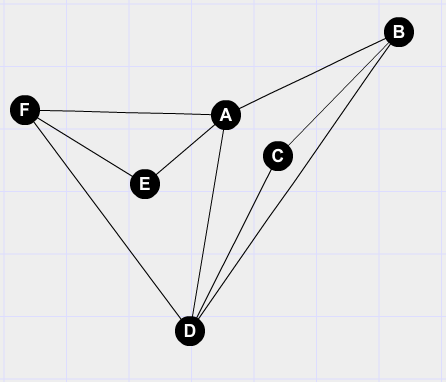
\includegraphics[width=5cm]{graphe1.png} }}%
				\qquad
				\subfloat[Après coloriage]{{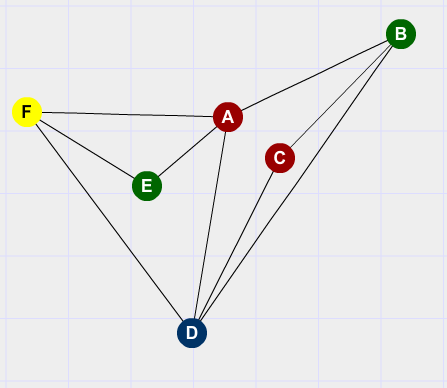
\includegraphics[width=5cm]{graphe1_c.png} }}%
				\caption{Graphe 1}%
				\label{fig:graphe1}%
			\end{figure}
		\end{itemize}
		\item Graphe 2, qui est un graphe dont le degré de chaque sommet vaut 5 :
		\begin{itemize}
			\item Temps moyen d'exécution : 0.0006128 secondes
			\item Représentation :
			\begin{figure}[h]%
				\centering
				\subfloat[Avant coloriage]{{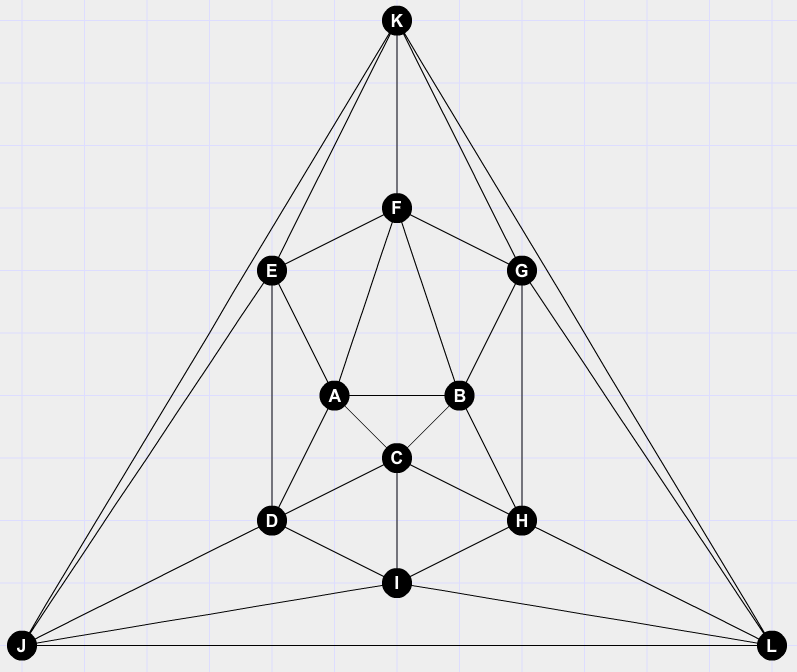
\includegraphics[width=5cm]{graphe2.png} }}%
				\qquad
				\subfloat[Après coloriage]{{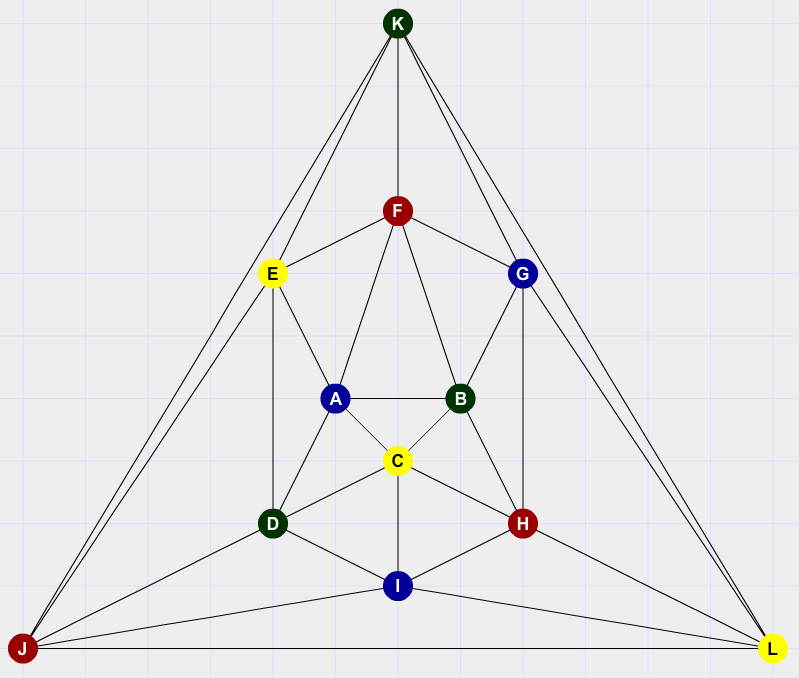
\includegraphics[width=5cm]{graphe2_c.png} }}%
				\caption{Graphe 2}%
				\label{fig:graphe2}%
			\end{figure}
		\end{itemize}
		\newpage
		\item Graphe 3, qui est un graphe dont le degré de chaque sommet vaut 3 :
		\begin{itemize}
			\item Temps moyen d'exécution : 0.0004002 secondes
			\item Représentation :
			\begin{figure}[h]%
				\centering
				\subfloat[Avant coloriage]{{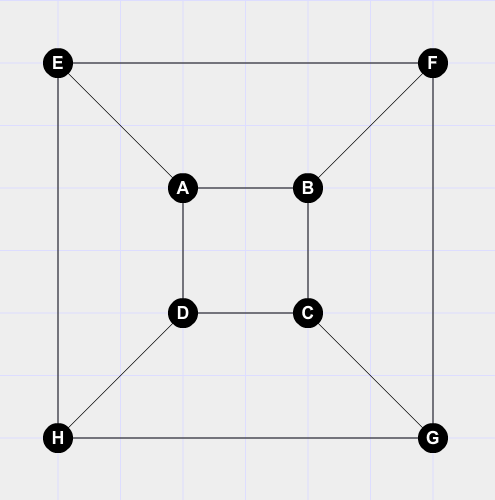
\includegraphics[width=5cm]{graphe3.png} }}%
				\qquad
				\subfloat[Après coloriage]{{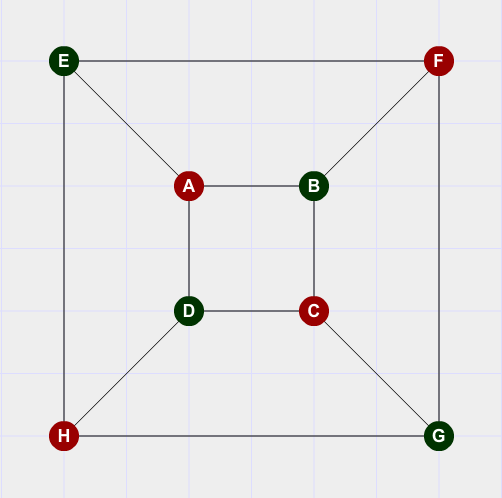
\includegraphics[width=5cm]{graphe3_c.png} }}%
				\caption{Graphe }%
				\label{fig:grphe3}%
			\end{figure}
		\end{itemize}
	\end{itemize}
	\newpage

	\section{Difficultés rencontrés}
	\paragraph{}
	Comme on l'a déjà dit dans l'introduction, le pseudo-code était un peu ambigu. Parfois les étapes étaient écrites explicitement, parfois on devait les déduire du contexte, ce qui a rendu la compréhension difficile. Par rapport à l'implémentation, l'étape la plus compliquée était de fusionner 2 sommets en un seul car il faut faire très attention à bien mettre à jour l'état de tous les voisins. C'est très facile de se tromper en travaillant avec des listes chaînées. Le débugger visuel était indispensable. En reste, il y avait un manque de confiance dans le code car on ne savait pas si on implémente les étapes correctement. En faisant une simulation entière sur papier nous a permis d'avoir une source de référence de l'état de la mémoire qu'on devait avoir à chaque étape.

	\section{Références}
	\begin{itemize}
		\item https://en.wikipedia.org/wiki/Five\_color\_theorem?fbclid=IwAR2gWXQwMi2bhCh9HIW6gnY\_vz\_qEf5Cwk5j-c-YYZk23LTf-KPZSMsBNJY
		\item http://cgm.cs.mcgill.ca/~athens/cs507/Projects/2003/MatthewWahab/5color.html
		\item http://mathonline.wikidot.com/5-colour-theorem-for-planar-graphs
	\end{itemize}
	
\end{document}\documentclass[a4paper, 11pt, oneside]{article}
